\documentclass[specialist,subf,href,colorlinks=true
%,times        % шрифт Times как основной
%,fixint=false % отключить прямые знаки интегралов
]{disser}
\usepackage[
  a4paper, mag=1000, includefoot,
  left=3cm, right=1.5cm, top=2cm, bottom=2cm, headsep=1cm, footskip=1cm
]{geometry}
\usepackage[T2A]{fontenc}
\usepackage[utf8x]{inputenc}
\usepackage[english,russian]{babel}
\usepackage{tikz}
\usepackage{listingsutf8}
\usepackage{listings}
\graphicspath{{images/}}
\definecolor{light-gray}{gray}{0.95}
\lstset{
  inputencoding=utf8x,
  extendedchars=\true,
  showstringspaces=false,
  basicstyle=\footnotesize,
  tabsize=2,
  backgroundcolor=\color{light-gray},
}
\usepackage{url}

%% Define a new 'leo' style for the package that will use a smaller font.
\makeatletter
\def\url@leostyle{%
  \@ifundefined{selectfont}{\def\UrlFont{\sf}}{\def\UrlFont{\small\ttfamily}}}
\makeatother
%% Now actually use the newly defined style.
\urlstyle{leo}
\begin{document}
\tableofcontents % это оглавление, которое генерируется автоматически
\intro
В последнее время наблюдается взрывной рост количества новых источников информации о генах, протеинах, химических исследованиях, лекарствах и болезнях. Растет при этом и разрозненность информации. Этот фактор приводит к тому, что результаты новых исследований просто теряются в море устаревших сведений.
Требуется совершить переход к новой модели хранения и обработки информации - Linked Data. Использование этой методологии существенно повысит связанность медицинских знаний, позволит открывать новые закономерности и получать новейшие данные об исследованиях.

Основная цель моей работы - это создание семантического хранилища медицинских знаний.
Для достижения поставленной цели решались следующие задачи:
\begin{enumerate}
\item Скачивание и парсинг информации с ресурса Webapteka
\item Разработка онтологии лекарственных препаратов
\item Конвертация html данных в rdf представление
\item Разработка SPARQL-запросов для извлечения информации и выявления дополнительных связей в RDF-хранилище.
\item Разработка пользовательского интерфейса
\item Кеширование элементов приложения для повышения производительности
\end{enumerate}

\chapter{Семантические сети}
\section{Введение в семантические сети}

Семантическая сеть (англ. Semantic Web) — это набор технологий, позволяющих представлять информацию в виде пригодном для машинной обработки: RDF, OWL, SPARQL. RDF используется для представления информации, SPARQL - для доступа к ней, OWL - добавляет метаинформацию, связи между концептами. \cite{linkeddata}

В RDF вся информация представляется в виде триплетов: субъект, предикат, объект. Триплеты по форме похожи на простое предложение.  Например:
\par Субъект: Александр
\par Предикат: Имеет пол
\par Объект: Мужской
\\Триплет может быть выражен в виде графа
\\
\par \begin{tikzpicture}[->, shorten >=1pt,auto,node distance=5cm,
  thick,main node/.style={circle,fill=blue!20,draw}]

  \node[main node] (2) {Александр};
  \node[main node] (4) [right of=2] {Мужской};

  \path[every node/.style={font=\sffamily\small}]
    (2) edge node {имеет пол} (4);
\end{tikzpicture}

Субъекты и объекты могут быть представлены URI, либо литералом. URI - это уникальный идентификатор, который обозначает сущность: например URI для собаки может быть таким \textit{'http://example.ru/animals/dog'}. Литерал - это просто строка, например 'Jack Nickolson', с возможными добавлениями, указывающими язык, тип данных (поддерживаемый XML, такие как integer и datetime). В идеале между сущностями и URI составлено взаимно однозначное соответствие: каждый URI принадлежит только одной сущности и каждая сущность имеет только один URI.
Для обозначение предикатов всегда используются URI.

Использование URI в RDF облегчает нахождение документов, связанных с сущностью. Например, если кто-то(или чья-то программа) ищет информацию о собаках, то ему надо искать все триплеты содержащие URI \textit{http://www.example.ru/animals/dog}.

RDF-документ представляет собой набор триплетов. Его можно выразить в виде графа, если представить URI как вершины, а предикаты как ребра графа.

\par \begin{tikzpicture}[->, shorten >=1pt,auto,node distance=5cm,
  thick,main node/.style={circle,fill=blue!20,draw}]
  \node[main node] (2) {Александр};
  \node[main node] (3) [below of=2] {Казань};
  \node[main node] (1) [right of=3] {Татарстан};
  \node[main node] (4) [right of=2] {Мужской};

  \path[every node/.style={font=\sffamily\small}]
    (2) edge node {имеет пол} (4)
	edge node {живет в} (3)
    (3) edge node {столица} (1);
\end{tikzpicture}

Таким образом можно построить граф неограниченного размера.
RDF как язык для хранилища имеет ряд преимуществ:
\begin{enumerate}
\item Простое агрегирование данных. Необходимо только добавить триплеты с указанием связи между сущностями.
\item Использование URI дает возможность объединять информацию о сущности с нескольких источников данных.
\item Поскольку RDF не имеет жестких, заведомо заданных требований к структуре данных, к наличию или отсутствию свойства, повышается плотность хранения информации.
\item RDF предлагает единый язык для представления практически любого знания.
\end{enumerate}
\section{OWL}
Технологии Semantic Web дают возможность выводить новые факты из базовых фактов, хранящихся в RDF. OWL добавляет к RDF информацию о классах, типах, логических зависимостях, доменов у свойств, пространстве возможных значений. \cite{soloviev}
\section{SPARQL}
SPARQL - язык запросов к RDF-хранилищу. SPARQL, как и большинство языков такого типа, содержит переменные в тексте запроса, в которые подставляются извлеченные данные.
Запрос вида
\begin{lstlisting}
SELECT ?x WHERE {
?x <http://www.example.com/has-gender> <http://www.example.com/male> . 
}
\end{lstlisting}
найдет все триплеты с указанным предикатом и объектом(ИМЕЕТ ПОЛ, МУЖСКОЙ) и вернет список субъектов. Информация возвращается в XML-формате.

Запрос может быть построен из нескольких триплетов. В следующем примере кода две конструкции, которые должны вернуть всех людей мужского пола.
\begin{lstlisting}
SELECT ?x WHERE {
?x <http://www.example.com/has-gender> <http://www.example.com/male> .
?x <http://www.example.com/has-species> <http://www.example.com/human> .
}
\end{lstlisting}
Это тип запросов основной в SPARQL. Хотя SPARQL беднее по функциональности чем SQL, он поддерживает схожий функционал для уточнения запроса: сортировка результатов, получение подмножества результатов, удаление дубликатов и т.д.
Следующий запрос вернет всех мужчин, которые имеют больше, чем 20 книг и, если имеется информация о предпочтениях в еде, она вернется тоже.
\begin{lstlisting}
PREFIX ex: <http://www.example.com/>
SELECT ?x ?foods WHERE {
?x ex:has-gender ex:male .
?x ex:has-species ex:human .
?x ex:has-book-count ?bookcount .
FILTER (?bookcount < 20)
}
OPTIONAL {
?x ex:likes-food ?foods .
}
}
\end{lstlisting}
Преимущества, которые могут быть получены за счет использования этого языка запросов понятны: человек или компьютер могут соединиться с любым открытым репозиторием, сделать очень специфичный запрос и получить машино-обрабатываемые данные.
\chapter{Сравнение RDF с другими моделями хранилищ}
В любом хранилище данных, доступ к информации осуществляется в соответствии с некоторой моделью, логической концепцией. В этой главе описываются модели хранения данных, использующиеся в настоящее время. Исследуются сходства RDF-модели с остальными и определяется, в какой степени подходы для традиционных баз данных применимы к RDF-хранилищам.

\section{Реляционные хранилища}
Эта модель была предложена в 1970г. Э.Коддом. В этом подходе теория множеств и логика предикатов используются для определения логической структуры хранилища данных и операций, которые могут быть к нему применены. В часности, разделяются логическая структура и физическая. СУБД может выбрать любой способ физического хранения данных, но то, как информация отображается пользователю, остается неизменным.

Реляционная модель описывает данные в терминах реляций, состоящих из неограниченного числа кортежей и аттрибутов. Реляции в целом схожи с таблицами, состоящих из строк и столбцов. Каждый кортеж является уникальным (ведь не имеет смысла один и тот же факт дважды).  Запросы к СУБД пишутся на декларативном языке, позволяющим пользователям указать, какие данные они хотят получить, не заставляя их указывать, каким способом это сделать. Как правило, это ответственность СУБД сделать запрос как можно более быстрым. Компонент, который выполняет оптимизацию, называется оптимизатором запросов.

Реляционная модель предназначена для поддержки запросов с перекрестными ссылками между блоками данных: 
\textit{
  'Получить всех механиков, которые работали над машиной, содержащей деталь X.'
}

\section{Key-Value хранилища(NoSQL)}
Имеют ряд существенных отличий от реляционных хранилищ:
\begin{enumerate}
\item В этой модели записи идентифицируются по ключу, при этом каждая запись имеет динамический набор атрибутов, связанных с ней.
\item Вместо реляций вводится понятие домена. Для доменов можно провести аналогию с таблицами, однако в отличие от таблиц для доменов не определяется структура данных. Домен – это коробка, в которую можно складывать все что угодно. Записи внутри одного домена могут иметь разную структуру.
\item В некоторых реализациях атрибуты могут быть только строковыми. В других реализациях атрибуты имеют простые типы данных, которые отражают типы, использующиеся в программировании: целые числа, массива строк и списки.
\item Между доменами, также как и внутри одного домена, отношения явно не определены.
\end{enumerate}

Хранилища типа ключ-значение ориентированы на работу с записями. Это значит, что вся информация, относящаяся к данной записи, хранится вместе с ней. Домен  может содержать бессчетное количество различных записей. Например, домен может содержать информацию о клиентах и о заказах. Это означает, что данные, как правило, дублируются между разными доменами. Это приемлемый подход, поскольку дисковое пространство дешевоe. Главное, что он позволяет все связанные данные хранить в одном месте, что улучшает масштабируемость, поскольку исчезает необходимость соединять данные из различных таблиц. При использовании реляционной БД, потребовалось бы использовать соединения, чтобы сгруппировать в одном месте нужную информацию.

Хотя для хранения пар ключ-значение потребность в отношения резко падает, отношения все же нужны. Такие отношения обычно существуют между основными сущностями. Например, система заказов имела бы записи, которые содержат данные о покупателях, товарах и заказах. При этом неважно, находятся ли эти данные в одном домене или в нескольких. Вместо этого, запись о заказе должна содержать ключи, которые указывают на соответствующие записи о покупателе и товаре. Поскольку в записях можно хранить любую информацию, а отношения не определены в самой модели данных, система управления базой данных не сможет проконтролировать целостность отношений. Это значит, что можно удалять покупателей и товары, которые они заказывали. Обеспечение целостности данных целиком ложится на приложение.

Сравнение key-value хранилищ и реляционных:
Доступ к данным
\\\begin{tabular}{p{0.45\linewidth}|p{0.45\linewidth}}
\hline
Реляционная\ БД & Хранилище типа ключ-значение  \\
\hline
Данные создаются, обновляются, удаляются и запрашиваются с использованием языка структурированных запросов (SQL). &
Данные создаются, обновляются, удаляются и запрашиваются с использованием вызова API методов. \\
\hline
SQL-запросы могут извлекать данные как из одиночной таблица, так и из нескольких таблиц, используя при этом соединения (join’ы). &
Некоторые реализации предоставляют SQL-подобный синтаксис для задания условий фильтрации. \\
\hline
SQL-запросы могут включать агрегации и сложные фильтры. &
Зачастую можно использовать только базовые операторы сравнений (=, !=, <, >, <= и =>). \\
\hline
Реляционная БД обычно содержит встроенную логику, такую как триггеры, хранимые процедуры и функции. &
Вся бизнес-логика и логика для поддержки целостности данных содержится в коде приложений. \\
\hline
\end{tabular}

Взаимодействие с приложениями
\\ \begin{tabular}{p{0.45\linewidth}|p{0.45\linewidth}}
\hline
Реляционная\ БД & Хранилище типа ключ-значение  \\
\hline
Чаще всего используются собственные API, или обобщенные, такие как OLE DB или ODBC. &
Чаще всего используются SOAP и/или REST API, с помощью которых осуществляется доступ к данным. \\
\hline
Данные хранятся в формате, который отображает их натуральную структуру, поэтому необходим маппинг структур приложения и реляционных структур базы. &
Данные могут более эффективно отображаться в структуры приложения, нужен только код для записи данных в объекты. \\
\hline
\end{tabular}

Преимущество хранилищ типа ключ-значение состоит в том, что они проще, а значит обладают большей масштабируемостью, чем реляционные БД. Такие хранилища легко и динамически расширяются. Но, в свою очередь, ограничения в реляционных БД гарантируют целостность данных на самом низком уровне. Данные, которые не удовлетворяют ограничениям, физически не могут попасть в базу. В хранилищах типа ключ-значение таких ограничений нет, поэтому контроль целостности данных полностью лежит на приложениях. Однако в любом коде есть ошибки. Если ошибки в правильно спроектированной реляционной БД обычно не ведут к проблемам целостности данных, то ошибки в хранилищах типа ключ-значение обычно приводят к таким проблемам.

Другое преимущество реляционных БД заключается в том, что они вынуждают вас пройти через процесс разработки модели данных. Если вы хорошо спроектировали модель, то база данных будет содержать логическую структуру, которая полностью отражает структуру хранимых данных, однако расходится со структурой приложения. Таким образом, данные становятся независимы от приложения. Это значит, что другое приложение сможет использовать те же самые данные и логика приложения может быть изменена без каких-либо изменений в модели базы. Чтобы проделать то же самое с хранилищем типа ключ-значение, попробуйте заменить процесс проектирования реляционной модели проектированием классов, при котором создаются общие классы, основанные на естественной структуре данных.

\section{RDF-хранилища}
RDF-системы баз данных относятся к типу NoSQL моделей, основанных на графах. Ключевые отличия от других реализаций \cite{rdfdiff}:
\begin{enumerate}
 \item Поддерживают спецификацию W3C - Linked Data. 
 \item Мощный стандартный язык запросов. NoSQL базы данных в основном не предоставляют высокоуровненого декларативного языка запросов, аналогичного SQL. Запросы в таких базах данных основываются на программной модели хранимой информации и языке реализации. SPARQL - очень большое преимущество RDF-хранилищ, обеспечивающее стандартизированный и совместимый язык с мощным функционалом. 
 \item Стандартизированный формат данных. Все RDF-хранилища поддерживают XML и N-Triples форматы данных.
 \item Простое объединение данных, источников данных. Так как RDF представляет собой перечень триплетов, для объединения данных необходимо только конкатенировать два списка. SPARQL язык поддерживает обращение к нескольким источникам в одном запросе.
 \item Содержат общедоступное описание схемы хранимой информации на декларативном языке OWL.
\end{enumerate}
 
Суммируя выше сказанное, RDF является оптимальным решением для организации сильно-распределенных хранилищ информации. 

\chapter{Разработка RDF-хранилища}

\section{Построение онтологии}
При построении RDF-хранилища, в первую очередь разрабатывается онтология - описание схемы данных хранилища на языке OWL. Уже существует множество полезных онтологий, части которых можно использовать в своей онтологии либо создавать на них ссылки.(проект http://swoogle.umbc.edu/ позволяет искать онтологии). Мощным средством для построения онтологий является Protege.

Основной класс в онтологии проекта - это Drug(лекарство). Большинство остальных классов образуют объектную часть предикатов.

Список свойств класса Drug:
\begin{enumerate}
 \item имеет международное название
 \item имеет торговое наименование
 \item принадлежит нескольким категориям
 \item имеет множество форм применения
 \item имеет фармакологию
 \item имеет множество показаний
 \item имеет множество противопоказаний
 \item имеет множество побочных эффектов
 \item имеет дозировку
 \item взаимодействует с другими лекарствами и группами лекарств
 \item содержит лекарственные ингридиенты
 \item имеет специальные указания
\end{enumerate}
В Protege онтология имеет следующий вид:
\\ 
\\ 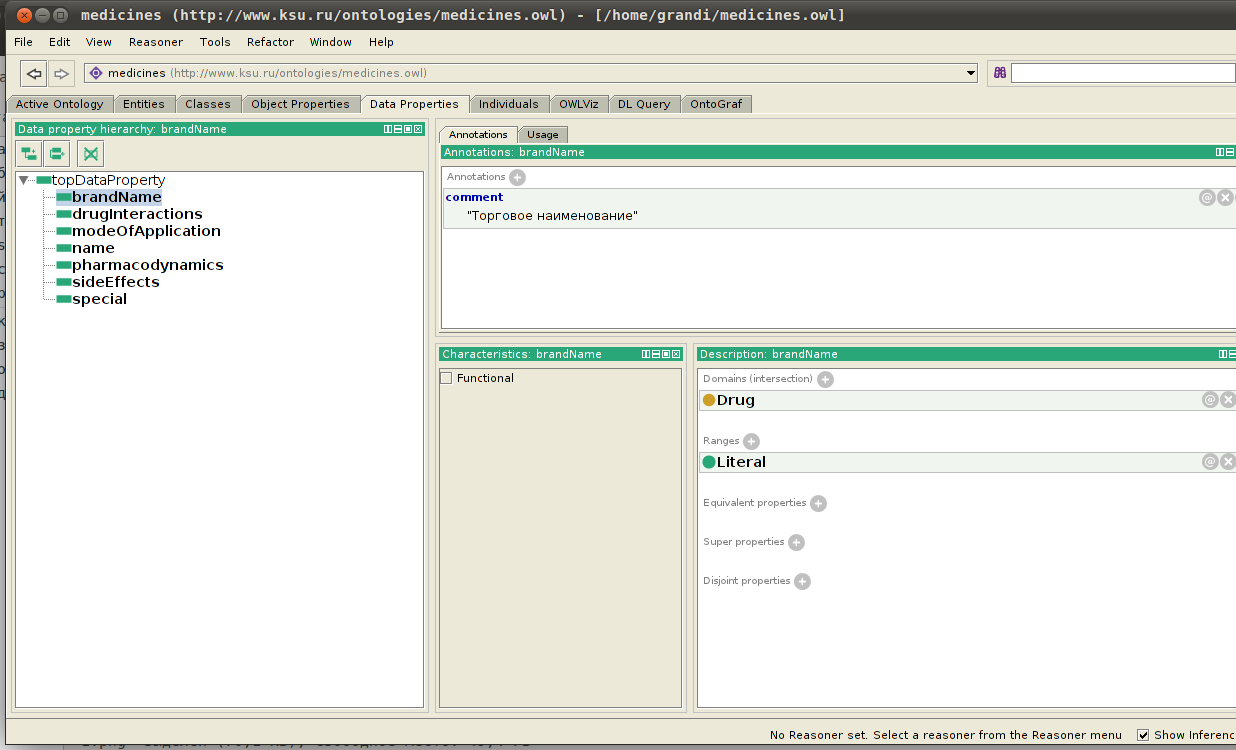
\includegraphics[width=160mm]{2.png}

\section{Выбор архитектуры и инструментов}

Ruby - мощный и гибкий язык. \cite{rubylang} Он предоставляет лаконичный синтаксис, возможность изменять классы и методы во время выполнения программы, на нем написано множество библиотек, существенно облегчающих построение Web-приложения. Руководствуясь этими соображениями, RDF-хранилище будет писаться на Ruby.

Существует несколько библиотек для работы с RDF-хранилищами, реализованных на Ruby. Основные отличия между ними – поддержка функций вывода, степень поддержки вывода для OWL, возможности использования в качестве точки доступа SPARQL, веб-доступ, возможность хранения четверок вместо триплетов, а так же поддержка хранилища языками программирования (наличие модулей). \cite{rubysem}

Кроме того, важным критерием является способность проецировать схему субъект-предикат-объект на экземпляр-свойство-значение, таким образом используя объектно-ориентированное программирование. Существуют, однако, глубинные различия объектов из ООП языков и RDF-объектами. Особенность RDF-сущностей в том, что они имеют URI, и они могут экземплярами нескольких классов. Для преодоления этой проблемы используется общая модель данных для ООП и RDF. В этой модели сущности могут иметь методы и свойства, должны иметь URI и могут быть экземплярами нескольких классов. Таким образом сочетаются возможности ООП и RDF.

Для использования в проекте, выбрана библиотека RDFrb. Она предоставляет наиболее обширный диапазон возможностей, и, что важно с иследовательской точки зрения, предоставляет абстрактный класс для переопределения функций хранилища. \cite{rdfrb}

Web-сервер будет базироваться на Ruby on Rails - фреймворке, написанном на Ruby, предоставляющем возможности xml-сериализации, html-парсинга, кеширования, REST-архитектуры.
\section{RDFrb}
RDFrb - библиотека для работы с семантическими данными. Для создания семантического графа нужно только указать онтологию и перечислить триплеты.
\begin{lstlisting}
  include RDF
  MyOnt = RDF::Vocabulary.new("http://ricardolopes.net/myont.owl#")
  graph = RDF::Graph.new
  items.each do |item|
    graph << [item["uri"], RDF.type, MyOnt.Item]
    graph << [item["uri"], MyOnt.hasName, item["name"]]
  end
  return graph
\end{lstlisting}
В этом примере предполагается, что у нас есть онтология с URI 
\\ \textit{'http://ricardolopes.net/myont.owl'}, которая содержит по меньшей мере класс Item и свойство hasName.
\\Теперь сохраним граф в N-Triples формате:
\begin{lstlisting}
  RDF::Writer.open("data/graph.nt") do |writer|
    graph.each_statement do |stmt|
      writer << stmt
    end
  end
\end{lstlisting}

\section{SPARQL-точка}
RDFrb дает возможность писать запросы к RDF-хранилищу как на чистом Ruby, так и на языке SPARQL. Для организации внешнего доступа к SPARQL-точке был добавлен роут по адресу /sparql, который получает GET-параметром текста запроса и возвращает ответ RDF-хранилища в XML-формате.
Также было написано несколько SPARQL-запросов для получения данных из RDF-хранилища внутри приложения.
\subsection{Получение списка всех лекарств}
Лекарство называются те сущности, которые имеют тип \textit{Лекарство}. SPARQL запрос выглядит так:
\begin{lstlisting}[language=SQL]
SELECT DISTINCT ?drug 
  WHERE {
    ?drug <#{RDF.type}> <#{@type}>
  }
}
\end{lstlisting}
\textit{\@type} - переменная экземпляра, которая содержит его RDF-тип. 
\subsection{Нахождение списка похожих лекарств}
Похожими считаются лекарства, у которых есть одинаковый компонент. SPARQL запрос выглядит так:
\begin{lstlisting}[language=SQL]
  SELECT ?drug 
  WHERE {
    ?drug <http://osmanov.me/drugComponent> ?drugPart .
    <#{uri}> <http://osmanov.me/drugComponent> ?drugPart
    FILTER (?drug != <#{uri}>)
  }
\end{lstlisting}
Оператор FILTER в запросе убирает из списка похожих препаратов само лекарство.
\subsection{Получение списка названий лекарств}
Запрашивается список всех литералов, являющихся объектной частью в триплетах вида: \textit{Лекарство имеет имя ...} SPARQL запрос выглядит так:
\begin{lstlisting}[language=SQL]
  SELECT DISTINCT ?drugname 
  WHERE {
	  ?drug <#{FOAF.name}> ?drugname
  }
\end{lstlisting}
\subsection{Получение списка суммарных противопоказаний для группы лекарств}
Запрос получается конкатенированием условий от каждого лекарства. Метод выглядит так:
\begin{lstlisting}[language=Ruby]
names_query = drugs.map do |drugname|
  "{ ?drug <#{FOAF.name}> '#{drugname}' }"
end.join(" UNION ")
query = "
  SELECT ?effects
  WHERE {
    #{names_query} .
    ?drug <http://osmanov.me/has_contraindication> ?effects
  }
"
sparql_query(query).map(&:effects).join(",")
\end{lstlisting}
\subsection{Получение списка суммарных побочных эффектов для группы лекарств}
Запрос получается конкатенированием условий от каждого лекарства. Метод выглядит так:
\begin{lstlisting}[language=Ruby]
names_query = drugs.map do |drugname|
  "{ ?drug <#{FOAF.name}> '#{drugname}' }"
end.join(" UNION ")
query = "
  SELECT ?toxicity
  WHERE {
    #{names_query} .
    ?drug <http://osmanov.me/has_toxicity> ?toxicity
  }
"
sparql_query(query).map(&:toxicity).join(",")
\end{lstlisting}

\section{Spira}
Spira - это RDF ORM(фреймфорк для представления информации, хранящейся в RDF-хранилище, в виде объектов). \cite{spira}
С его использованием создается Ruby-класс Drug. Экземпляр этого класса содержит значения всех триплетов для сущности, которую он отображает.
Для этого в заголовке добавляем информацию о хранимых аттрибутах.
\begin{lstlisting}[language=Ruby]
include Spira::Resource
base_uri "http://osmanov.me/drugs/"
type URI.new("http://osmanov.me/drugs")
property :intern_title, 
  :predicate => URI.new("http://osmanov.me/intern_title"), 
  :type => String
property :brandName,  
  :predicate => FOAF.name, 
  :type => String
has_many :drugCategories, 
  :predicate => URI.new("http://osmanov.me/has_drug_category"), 
  :type => :DrugCategory
has_many :dosageForms, 
  :predicate => URI.new("http://osmanov.me/has_dosage_form"),
  :type => String
property :pharmacology, 
  :predicate => URI.new("http://osmanov.me/has_pharmacology"), 
  :type => String
has_many :indications, 
  :predicate => URI.new("http://osmanov.me/has_indication"), 
  :type => String
has_many :contraindications, 
  :predicate => URI.new("http://osmanov.me/has_contraindication"), 
  :type => String
has_many :sideEffects, 
  :predicate => URI.new("http://osmanov.me/has_side_effects"), 
  :type => String
property :dosage, 
  :predicate => URI.new("http://osmanov.me/dosage"), 
  :type => String
has_many :interactions, 
  :predicate => URI.new("http://osmanov.me/has_interactions"), 
  :type => :DrugInteraction
has_many :drugParts, 
  :predicate => URI.new("http://osmanov.me/drugComponent"), 
  :type => :DrugPart
property :special, 
  :predicate => URI.new("http://osmanov.me/special"), 
  :type => String
\end{lstlisting}


\chapter{Заполнение RDF хранилища}
\section{Парсинг интернет-ресурса Web-аптека}
Для наполнения RDF-хранилища использовался ресурс \textit{http://webapteka.ru}. Страница лекарства имеет URL вида \textit{http://webapteka.ru/drugbase/name1.html}, вид ее представлен на рисунке.
\\ 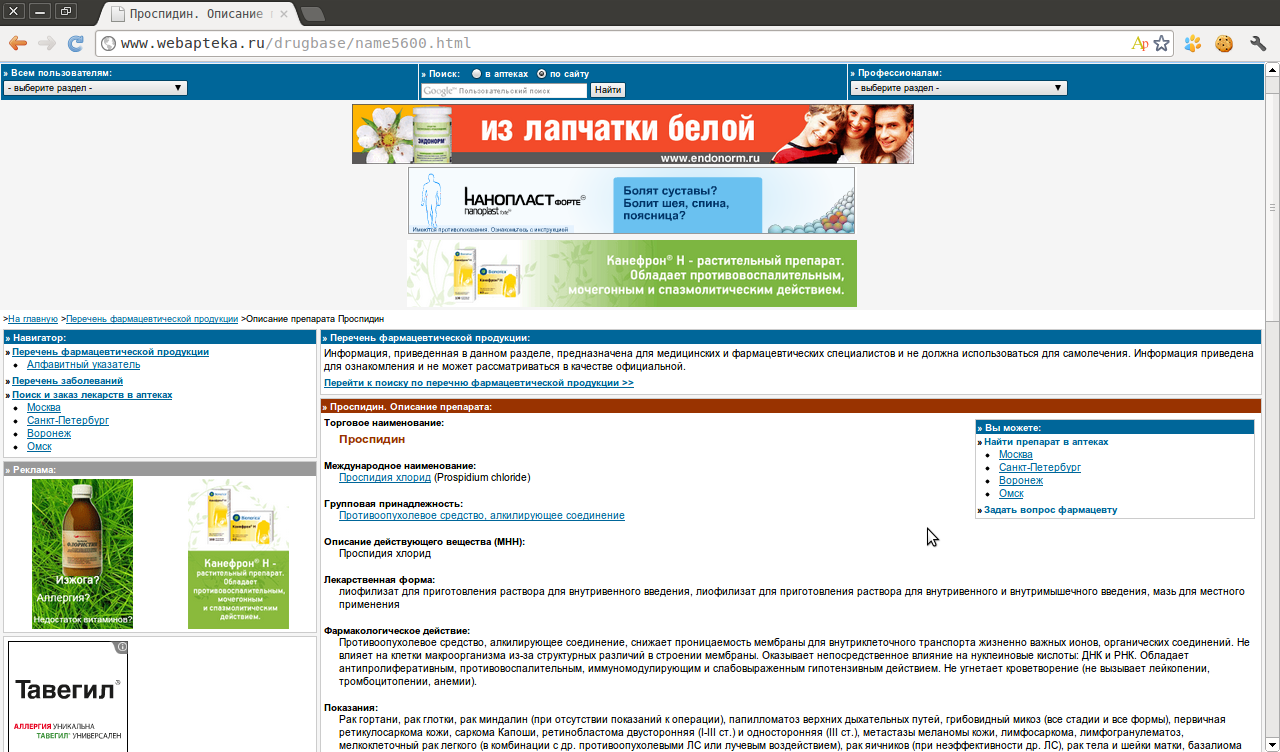
\includegraphics[width=160mm]{3.png}
\\Для получения базы лекарств необходимо пройти в цикле по всем URL, подставляя значение итератора как номер лекарства и распознать информацию.

Страница представляет собой HTML с inline-стилями, семантические блоки не обозначены классами. Поэтому расположение требуемой информации идентифицировалось по стилям, оформляющего его блока. Для построения DOM-дерева документа и поиску по нему использовалась библиотека Nokogiri. \cite{nokogiri}

Теперь для того, чтобы получить DOM-элемент необходимо только указать его CSS-путь или XPATH-путь. Так, например, выделяется блок с информацией о лекарстве:
\begin{lstlisting}
 doc.xpath("//div[@style='_width:100%; padding:5px; clear:left']").first
\end{lstlisting}
Названия свойств лекарства выделены жирным шрифтом:
\begin{lstlisting}
 table.css("b").first
\end{lstlisting}
Сами свойства имееют сдвиг влево на 20px:
\begin{lstlisting}
 table.xpath(".//div[@style='margin-left:20px']")
\end{lstlisting}
Распознанная информация сохраняется в файл в формате YAML.
\section{Сохранение информации в RDF-формате}
Как итог парсинга ресурса Webapteka получается файл в формате YAML, содержащей таблицы сопоставления свойства и его названия для каждого лекарства. Для того, чтобы преобразовать эти данные в формат RDF, был написан скрипт, создающий записи в RDF хранилище и ставящий в соответствие записи из YAML-файла и новыми записями.

Свойства примитивного типа данных просто копируются в свойство у Spira-модели. Те же свойства, которые описывают отношение один-ко-многим разбиваются на части, обозначающие название семантической единицы.

Так записывается торговое название лекарства:
\begin{lstlisting}[language=Ruby]
 drug_in_base.brandName = drug["Торговое наименование"]
\end{lstlisting}
А так список групп, к которым оно принадлежит:
\begin{lstlisting}[language=Ruby]
  groupName = drug["Групповая принадлежность"]
  if groupName
    if drugCategories[groupName]
      drugCategory = DrugCategory.for(drugCategories[groupName])
    else
      drugCategory = DrugCategory.for(drugCategoryID)
      drugCategories[drug["Групповая принадлежность"]] = drugCategoryID
      drugCategoryID += 1
    end
    drugCategory.name = groupName
    drugCategory.save!
    drug_in_base.drugCategories.merge([drugCategory])
  end
\end{lstlisting}


\chapter{Построение web-интерфейса}
Для прототипирования web-интерфейса в последнее время зачастую используются CSS-фреймворки. В моем проекте использовался Bootstrap. Его преимущества:
\begin{enumerate}
 \item 12-столбцовая сетка
 \item Jquery-плагины
 \item Поддержка LESS
\end{enumerate}
\section{Главная страница}
Главная страница содержит список всех лекарств и навигационную часть. 
\\ 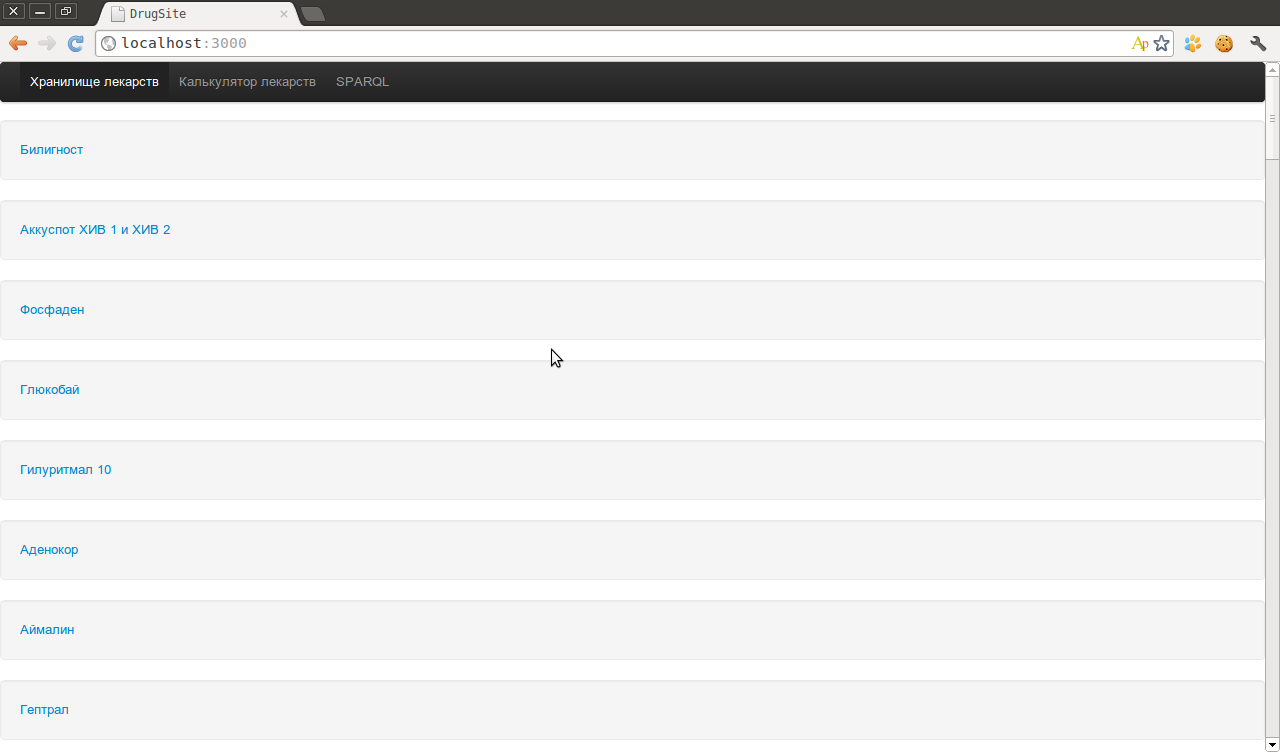
\includegraphics[width=160mm]{4.png}

Согласно правилам оформления Bootstrap, навигация обрамляется блоками navbar, navbar-inner и container.
\lstinputlisting[language=HTML]{code/main_page_fragment.html}

Для выделения строки с названием лекарства, обрамляющему параграфу добавлен класс \textit{well}.
\begin{lstlisting}[language=HTML]
<p class="well">
  <a href="/drugs/36">Билигност</a>
</p>
\end{lstlisting}

\section{Страница препарата}
На странице лекарства, помимо навигационной части, присутствует располосованная таблица со свойствами препарата.
\\ 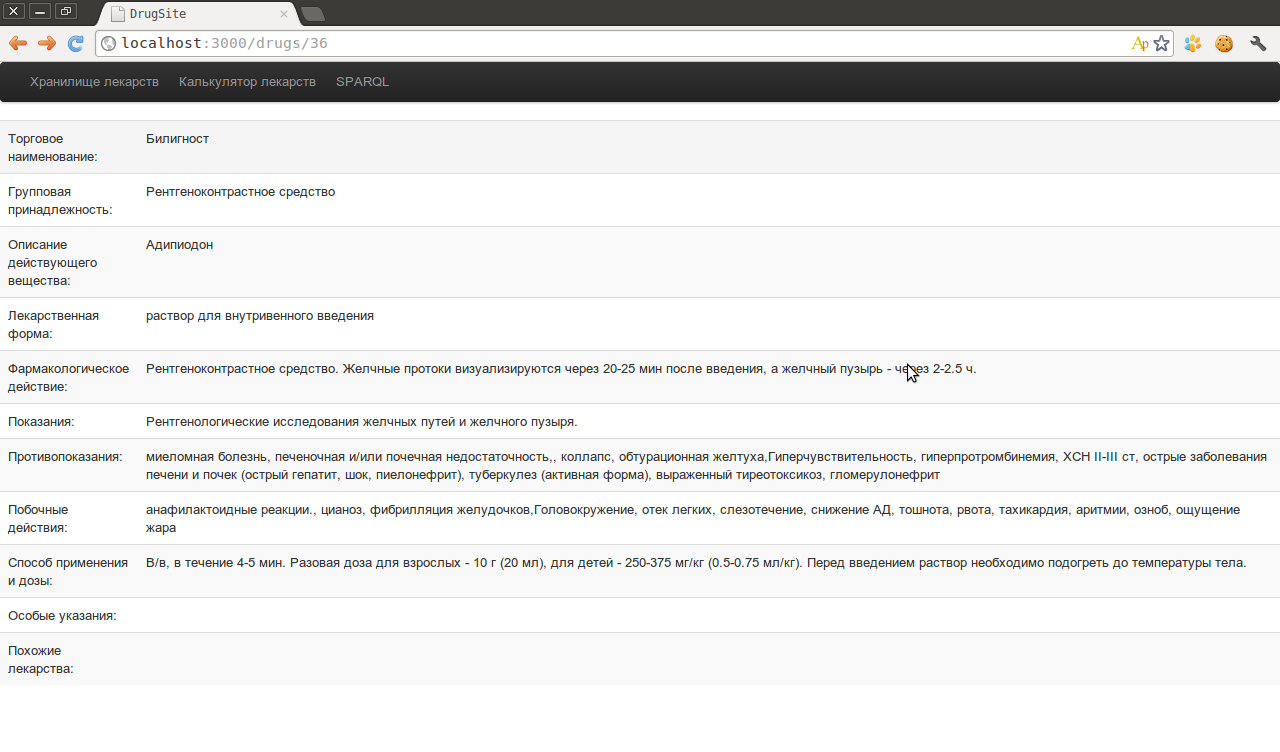
\includegraphics[width=160mm]{5.png}
\\ Этот эффект достигается путем добавления классов \textit{table} и \textit{table-striped} к таблице.
\begin{lstlisting}[language=HTML]
 <table class="table table-striped">
\end{lstlisting}

\section{Калькулятор лекарств}
На этой странице присутствует форма с текстовым полем для ввода названия лекарства и два блока, в которую выводится полученная информация.
\\ 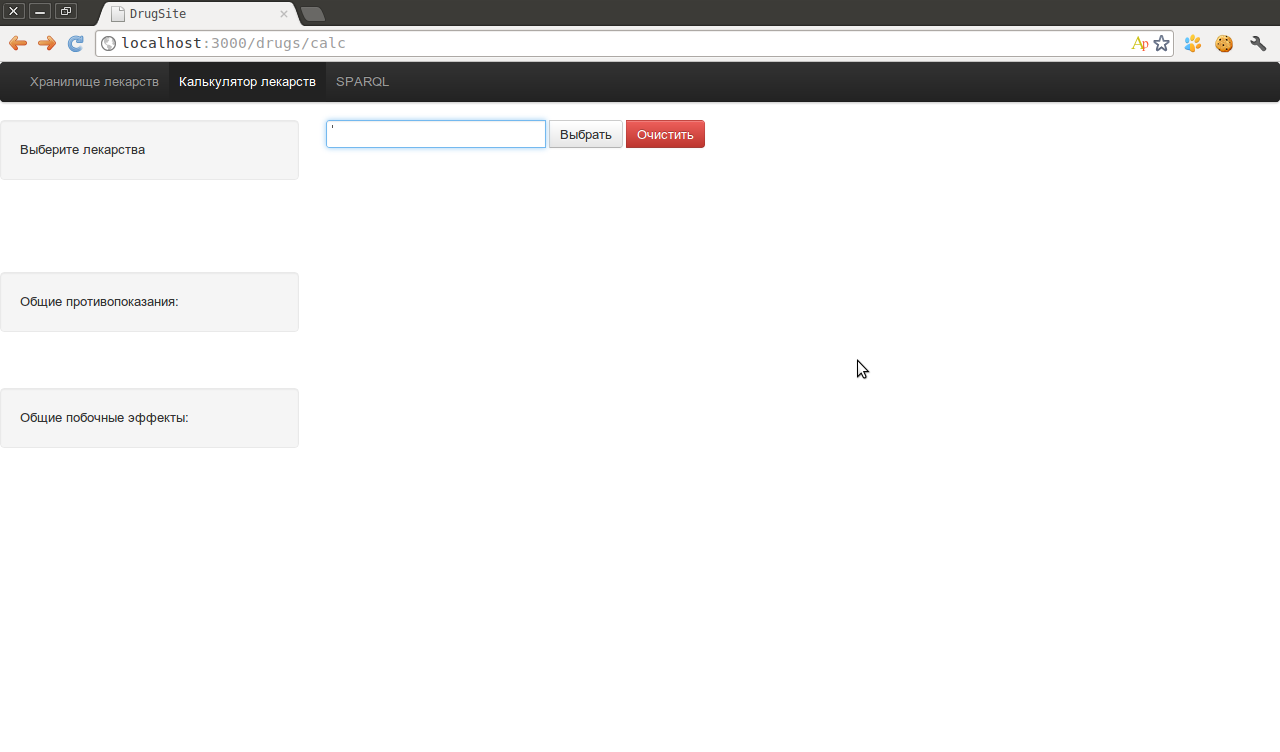
\includegraphics[width=160mm]{7.png}
\\ Вводимое название лекарства дополняется автоматически.
\\ 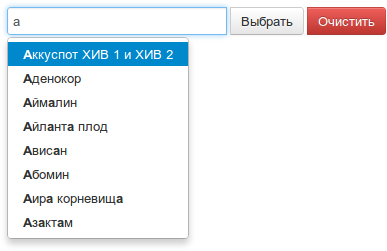
\includegraphics[width=90mm]{6.png}
\\Для данного функционала использовался плагин \textit{typeahead}. Чтобы его использовать, надо передать в функцию typehead массив возможных названий и идентификатор текстового поля.
\begin{lstlisting}
$(".select_drugs #drugs").typeahead({
  source: <%= raw @drug_names.inspect %>
});
\end{lstlisting}
После выбора названия препарата, осуществляется ajax-запрос к серверу. Отправляется список выбранных лекарств, возвращается список общих противопоказаний и побочных эффектов.
Для этого написаны две javascript-функции:
\begin{lstlisting}
selected_drugs = [];
var getContraIndications = function(drugs){
  $.get("<%= effects_drugs_path %>", {
    type: 'contraindications',
    drugs: selected_drugs
  }, function (response) {
    $(".contra-indications").text(response);
  });
};

var getToxicities = function(drugs){
  $.get("<%= effects_drugs_path %>", {
    type: 'toxicities',
    drugs: selected_drugs
  }, function (response) {
    $(".toxicities").text(response);
  });
};

$(".select_drugs .btn").click(function(e){
  e.preventDefault();
  var drug_name = $(".select_drugs #drugs").val();
  if (drug_name == "") {
    return false;
  };
  selected_drugs.push(drug_name);
  $(".selected_drugs").append("<li>" + drug_name + "</li>")
  $(".select_drugs #drugs").val("")
  getContraIndications(selected_drugs);
  getToxicities(selected_drugs);
});
\end{lstlisting}

После нажатия на кнопку \textit{Очистить} удаляется содержимое списка выбранных лекарств и блоков с информацией о противопоказаниях и побочных эффектах:
\begin{lstlisting}
$(".select_drugs .clear_selected_drugs").click(function(e){
  selected_drugs = [];
  $(".selected_drugs").html("");			
  $(".contra-indications").html("");
  $(".toxicities").html("")
  e.preventDefault();
});
\end{lstlisting}

Кнопки оформлены стилями \textit{btn} и \textit{btn-danger}
\begin{lstlisting}[language=HTML]
<button class="btn" href="#">Выбрать</button>
<button class="btn btn-danger clear_selected_drugs" href="#">Очистить</button>
\end{lstlisting}

\section{SPARQL форма}
Страница содержит форму для отправки SPARQL-запросов к серверу.
\\ 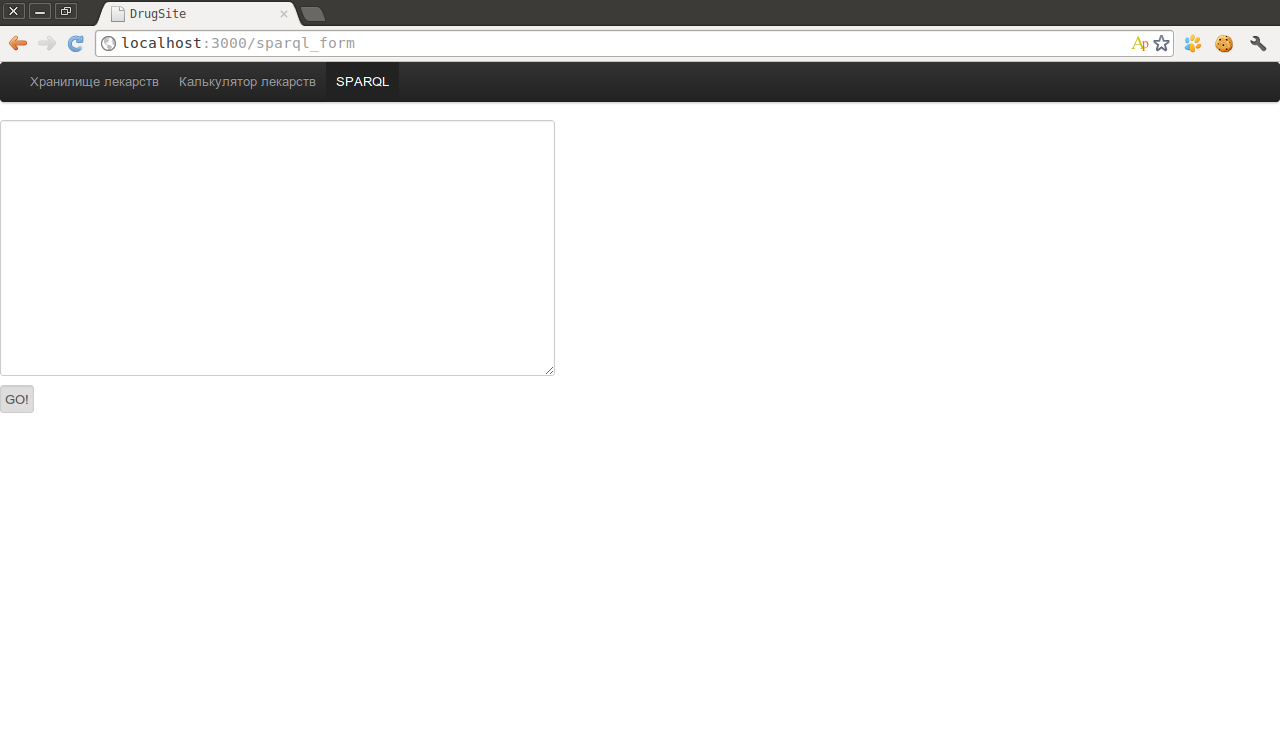
\includegraphics[width=160mm]{8.png}

\addcontentsline{toc}{chapter}{Заключение}
\chapter*{Заключение}
В данной работе представлены и проанализированы все этапы современной разработки RDF-хранилища:
\begin{enumerate}
 \item Построение онтологии
 \item Распознавание и подготовка данных для RDF-хранилища.
 \item Заполнение RDF-хранилища.
 \item Написание SPARQL-запросов, реализация SPARQL-точки.
 \item Построение пользовательского интерфейса.
\end{enumerate}
В реализованном RDF-хранилище представлено более 20000 лекарств, подготовлена система создания связей с другими RDF-хранилищами. Пользователи сайта могут получать информацию о лекарствах, недоступную на других ресурсах: суммарные противопоказания и побочные эффекты для группы лекарств, похожие препараты.

Данная система может использоваться как информационный ресурс для врачей и пациентов. Благодаря SPARQL-точке, хранилище может использоваться и как основа для семантических ризонеров.

\begin{thebibliography}{9}
  \bibitem {soloviev} Иванов В.В., Соловьев В.Д., Добров Б. В., Лукашевич Н.В., \emph{Онтологии и тезаурусы}, КГУ, 2008.
  \bibitem {linkeddata} T.Heath, C.Bizer, \emph{Linked Data: Evolving the Web into a Global Data Space}, Morgan \& Claypool, 2011.
  \bibitem {ricardolopes} R. Lopes, \emph{Developing for the Semantic Web with Ruby on Rails, the 2012 guide.}, \url{http://ricardolopes.net/blog/developing-for-the-semantic-web-with-ruby-on-rails-the-2012-guide/}
  \bibitem {spira} B. Lavender, \emph{Spira: A Linked Data ORM for Ruby.}, \url{http://blog.datagraph.org/2010/05/spira/}
  \bibitem {rdfdo} B. Lavender, \emph{RDF-do.}, \url{https://github.com/bhuga/rdf-do/}
  \bibitem {rubysem} V. Eisenberg, Y. Kanza, \emph{Ruby on Semantic Web}, \url{www.cs.technion.ac.il/~kanza/Papers/ ICDE11.pdf/}
  \bibitem {rubylang} D. Flanagan, Y. Matsumoto, \emph{The Ruby Programming Language.}, O’Reilly, 2008.
  \bibitem {rdfretr} A. Hertel, J. Broekstra, \emph{RDF Storage and Retrieval Systems},  Handbook on Ontologies, 2009.
  \bibitem {rdflatenc} A. Owens, \emph{Using Low Latency Storage to Improve RDF Store Performance},  University of Southampton, 2011.
  \bibitem {sparql} E. Prud'Hommeaux, \emph{SPARQL query language for RDF},  W3C working draft, 2008
  \bibitem {rdfdiff} A. Bendiken, \emph{How RDF Databases Differ from Other NoSQL Solutions.}, \url{http://blog.datagraph.org/2010/04/rdf-nosql-diff/}
  \bibitem {rdfrb} A.Bendiken, \emph{RDF.rb: Linked Data for Ruby}, \url{http://rdf.rubyforge.org/}
  \bibitem {nokogiri} A. Patterson, M. Dalessio, C. Nutter, \emph{Nokogiri: an HTML, XML, SAX, and Reader Parser}, \url{https://github.com/tenderlove/nokogiri}
\end{thebibliography}

\addcontentsline{toc}{chapter}{Листинг}
\chapter*{Листинг}
\addcontentsline{toc}{section}{Парсинг Webapteka}
\section*{Парсинг Webapteka}
\lstinputlisting[language=Ruby]{code/parser.rb}
\addcontentsline{toc}{section}{Настройка RDF-репозитория}
\section*{Настройка RDF-репозитория}
\lstinputlisting[language=Ruby]{code/repository.rb}
\addcontentsline{toc}{section}{Заполнение RDF-хранилища}
\section*{Заполнение RDF-хранилища}
\lstinputlisting[language=Ruby]{code/seeds.rb}
\addcontentsline{toc}{section}{Контроллеры}
\section*{Контроллеры}
\addcontentsline{toc}{subsection}{DrugsController}
\subsection*{DrugsController}
\lstinputlisting[language=Ruby]{code/drugs_controller.rb}
\addcontentsline{toc}{subsection}{SparqlController}
\subsection*{SparqlController}
\lstinputlisting[language=Ruby]{code/sparql_controller.rb}
\addcontentsline{toc}{section}{Модели}
\section*{Модели}
\addcontentsline{toc}{subsection}{Drug}
\subsection*{Drug}
\lstinputlisting[language=Ruby]{code/drug.rb}
\addcontentsline{toc}{subsection}{DrugCategory}
\subsection*{DrugCategory}
\lstinputlisting[language=Ruby]{code/drug_category.rb}
\addcontentsline{toc}{subsection}{DrugInteraction}
\subsection*{DrugInteraction}
\lstinputlisting[language=Ruby]{code/drug_interaction.rb}
\addcontentsline{toc}{subsection}{DrugPart}
\subsection*{DrugPart}
\lstinputlisting[language=Ruby]{code/drug_part.rb}
\addcontentsline{toc}{section}{Представления}
\section*{Представления}
\addcontentsline{toc}{subsection}{Основной слой}
\subsection*{Основной слой}
\lstinputlisting[language=HTML]{code/application.html.erb}
\addcontentsline{toc}{subsection}{Список лекарств}
\subsection*{Список лекарств}
\lstinputlisting[language=HTML]{code/index.html.erb}
\addcontentsline{toc}{subsection}{Страница лекарства}
\subsection*{Страница лекарства}
\lstinputlisting[language=HTML]{code/show.html.erb}
\addcontentsline{toc}{subsection}{Калькулятор лекарств}
\subsection*{Калькулятор лекарств}
\lstinputlisting[language=HTML]{code/calc.html.erb}
\end{document}
